\documentclass[conference]{IEEEtran}
\usepackage[T1]{fontenc}
\usepackage{amsmath,amssymb}
\usepackage{booktabs}
\usepackage{array}
\usepackage{graphicx}
\usepackage{url}
\usepackage{dblfloatfix}
\usepackage{capt-of}
\usepackage{balance}
\newcommand{\um}{\ensuremath{\mu\mathrm{m}^2}}
\title{STDM: A Shared Tangent-Plane FP32 Divider--Multiplier\\
with Multi-Level Accuracy--PPA Tradeoffs}
\author{\IEEEauthorblockN{Pingchuan Dong}}
\begin{document}
\maketitle

\begin{abstract}
Division and multiplication are often implemented as separate approximate
operators. This paper presents four STDM designs at accuracy levels L0--L3, each implementing approximate FP32 division and multiplication with a shared mantissa datapath. We derive the relation between their local tangent planes
and express both operations as two residual products and a constant.
Absorbing the divider's reciprocal scale into these coefficients removes a
subsequent multiplication. An exact recoding then replaces signed residual
products and subtraction with unsigned products and addition. At each accuracy level, DIV and MUL use the same two short multipliers and one adder. In a TSMC 65-nm implementation, sharing at levels L1--L3 reduces area by
17.2--19.0\%, power by 31.6--42.4\%, and area--delay product by 11.8--14.4\%
relative to matched separate cores. DIV-only comparisons with PACE, FPD2D, and PLSAD show the remaining tradeoff
between numerical accuracy and hardware cost. At L3, the complete shared unit
uses 92.5\% less area and 74.5\% less delay than an exact DesignWare FP32
DIV+MUL unit.
\end{abstract}

\begin{IEEEkeywords}
approximate computing, floating-point arithmetic, divider, multiplier,
tangent-plane approximation, arithmetic sharing
\end{IEEEkeywords}

\section{Introduction}
Approximate arithmetic can reduce computation cost when an application
tolerates numerical error. Division is a natural target because its mantissa
computation is expensive. With most prior works, approximate dividers and multipliers are optimized separately; as a result, processing element that issues one operation at a time carries two mantissa cores.

This duplication is particularly costly in area-constrained accelerators whose kernels use multiplication for updates or accumulations, and need division for normalization or scaling. For example, K-means computes distances and coordinate sums with multiplications, then divides each sum by its cluster
population to update the centroids~\cite{chen2010kmeans}. Normalized adaptive
filters similarly combine multiply-accumulate operations with a division by
the input energy~\cite{yao2024nlms}. STDM solves this problem by taking advantage of the similarity in the approximation formulae for multiplication and division, reducing the overall area, power, and delay. The operation is selected independently for each input, but one STDM unit performs either division or multiplication, not both simultaneously.

STDM is built on piecewise tangent plane approximation, as inspried by OAM, which approximates multiplication around the midpoint of each mantissa cell~\cite{chen2020oam}. We show that the
divider tangent plane at the same midpoint uses the same residual terms,
with one sign change and a reciprocal-square scale. After absorbing this scale
into the divider coefficients, both operations comprise two short products and a cell-selected constant.

A direct implementation still needs signed products and a conditional
subtraction. Exact recoding transfers the residual half-range into the constant
and complements the short divisor field in DIV mode. The result uses two
unsigned products and positive accumulation while preserving every retained
integer code.

STDM comprises four accuracy levels, L0--L3. The level is fixed when the circuit
is generated; an input selects the operation. We evaluate both standalone
dividers and matched separate and shared DIV+MUL cores.

The contributions are as follows:
\begin{itemize}
  \setlength{\itemsep}{0pt}
  \setlength{\parskip}{0pt}
  \setlength{\parsep}{0pt}
  \item We derive a common affine form that exposes the FP32 logic available
  for sharing.
  \item We absorb reciprocal-square scaling into divider coefficients and use
  an exact unsigned recoding to remove signed products and the DIV subtraction.
  \item We analyze partition, truncation, and coefficient error, and calibrate
  coefficients using the complete packed FP32 result.
  \item We compare identical-output shared and separate cores. At L1--L3,
  sharing saves 17.2--19.0\% area and 31.6--42.4\% power; DIV-only results
  quantify the cost against specialized dividers.
\end{itemize}

\section{Related Work}
Approximate dividers differ in which part of division they simplify.
Non-restoring and dynamic designs reduce the cost of quotient generation
through approximate cells or pruning
\cite{chen2015nonrestoring,hashemi2016dynamic}.
TruncApp combines precision reduction with an approximate divider
implementation~\cite{vahdat2017truncapp}. These approaches retain much of
the original arithmetic structure, so their cost depends strongly on the
retained width.

Logarithmic designs replace division with subtraction in an approximate
logarithm domain. FaNZeD, LEAD, and CADE use compensation or modified
approximations to improve the numerical result
\cite{saadat2019fanzed,ratnaparkhi2022lead,imani2019cade}.
Among the works reviewed here, SIMDive is the closest approximate combined
operator. It supports multiplication and division through shared
Mitchell log-domain arithmetic~\cite{ebrahimi2020simdive}, but processes
8--32-bit integers in SIMD FPGA lanes. STDM is a
scalar FP32 ASIC design whose measured cost includes
sign, exponent, normalization, and packing. Converting SIMDive into an FP32
unit would introduce an adapter not evaluated in the original paper and would
change both its numerical behavior and hardware cost. We therefore discuss
SIMDive as related work but do not use it as a PPA baseline.

Exact FP units have also combined multiplication and division to save
hardware, but they solve a different problem. Chen \emph{et al.} share
signed-digit adders, a termination multiplier, and normalization stages in a
single-precision fused unit~\cite{chen2004fused}; unlike STDM, its target is an
exact floating-point result rather than a selectable approximation level. The
DIVA FPU reuses a pipelined mantissa multiplier across Taylor-series divider
iterations~\cite{kwon2004diva}, so its cost is tied to a sequential schedule
rather than a one-pass combinational approximation. GRFPU similarly reuses
multiplication hardware for iterative division and square root and supports
both IEEE-754 single and double precision~\cite{gaislergrfpu}. Its formats,
operation set, and multicycle interface differ from STDM. These differences
prevent a controlled PPA comparison, so the exact designs are used only to
place arithmetic sharing in context.

Reciprocal designs approximate $1/y$ and combine it with the dividend.
SAADI-EC uses Taylor-series refinement, ILAFD combines reciprocal approximation
with logarithmic multiplication, and QIAD uses quadratic interpolation
\cite{melchert2019saadi,oelund2023ilafd,liu2023qiad}.
PACE expresses its piecewise reciprocal computation through shifts, additions,
and correction terms~\cite{wen2025pace}. This avoids general multipliers in
its divider mantissa core.

Surface-fitting designs approximate $x/y$ directly.
Earlier curve fitting, PLSAD, and FPD2D illustrate this approach
\cite{wu2015curve,wu2024plsad,dimeo2025fpd2d}.
PLSAD combines local fitting with simplified arithmetic; FPD2D optimizes
quantized coefficients over a two-dimensional mantissa partition.
They provide strong DIV-only baselines. STDM also evaluates a local affine
function, but derives its coefficients from related product and quotient
planes. That relation allows one datapath to serve both operations. The
evaluation separates this architectural benefit from standalone divider
efficiency.

\section{Related Divider and Multiplier Planes}
\subsection{Mantissa Partition and Tangent Planes}
For a normal finite FP32 input, write
$F_x=(-1)^{s_x}x2^{E_x}$, where $x\in[1,2)$~\cite{Ieee}.
The result sign is $s_x\oplus s_y$. The exponent calculation uses
$E_x+E_y$ for multiplication and $E_x-E_y$ for division, followed by
normalization. We focus on the mantissa functions $xy$ and $x/y$.

Level $n$ divides each axis of $[1,2)\times[1,2)$ into $2^n$ equal
intervals. The leading $n$ fraction bits identify indices $i_x,i_y$.
Their cell midpoints are
\begin{equation}
\begin{aligned}
k_x&=1+(i_x+\tfrac12)2^{-n},\\
k_y&=1+(i_y+\tfrac12)2^{-n}.
\end{aligned}
\label{eq:midpoints}
\end{equation}
We omit the level superscript when the selected cell is clear.
At L0, $k_x=k_y=3/2$. At L3 there are eight intervals per axis.
All L0--L3 midpoints have denominator at most 16, so midpoint representation
is exact.

Define centered residuals $r_x=x-k_x$ and $r_y=y-k_y$.
They satisfy $|r_x|,|r_y|\leq2^{-(n+1)}$.
The first-order expansions at the midpoint give
\begin{align}
\widehat m&=k_xk_y+k_yr_x+k_xr_y,\label{eq:mulplane}\\
\widehat d&=c(k_xk_y+k_yr_x-k_xr_y),
\quad c=k_y^{-2}.\label{eq:divplane}
\end{align}
Equation~\eqref{eq:mulplane} is the local OAM product plane.
Equation~\eqref{eq:divplane} follows from
$f_x(k_x,k_y)=1/k_y$ and $f_y(k_x,k_y)=-k_x/k_y^2$.
The two expressions have the same residual products and constant before
division applies $c$.

For completeness, expanding division in the original coordinates gives
\begin{equation}
\begin{aligned}
\widehat d
&=\frac{k_x}{k_y}+\frac{x-k_x}{k_y}
  -\frac{k_x(y-k_y)}{k_y^2}\\
&=\frac{k_xk_y+k_yx-k_xy}{k_y^2}.
\end{aligned}
\label{eq:directplane}
\end{equation}
The product plane in those coordinates is
$\widehat m=-k_xk_y+k_yx+k_xy$.
Thus both the constant and the $y$ term appear with different signs before
centering. Substituting $x=k_x+r_x$ and $y=k_y+r_y$ collects the midpoint
products into one positive constant. Only the residual $y$ term then changes
sign. This is the reason for using centered coordinates in the shared circuit.
Centering itself neither discards input bits nor changes the local plane.

\begin{figure}[t]
\centering
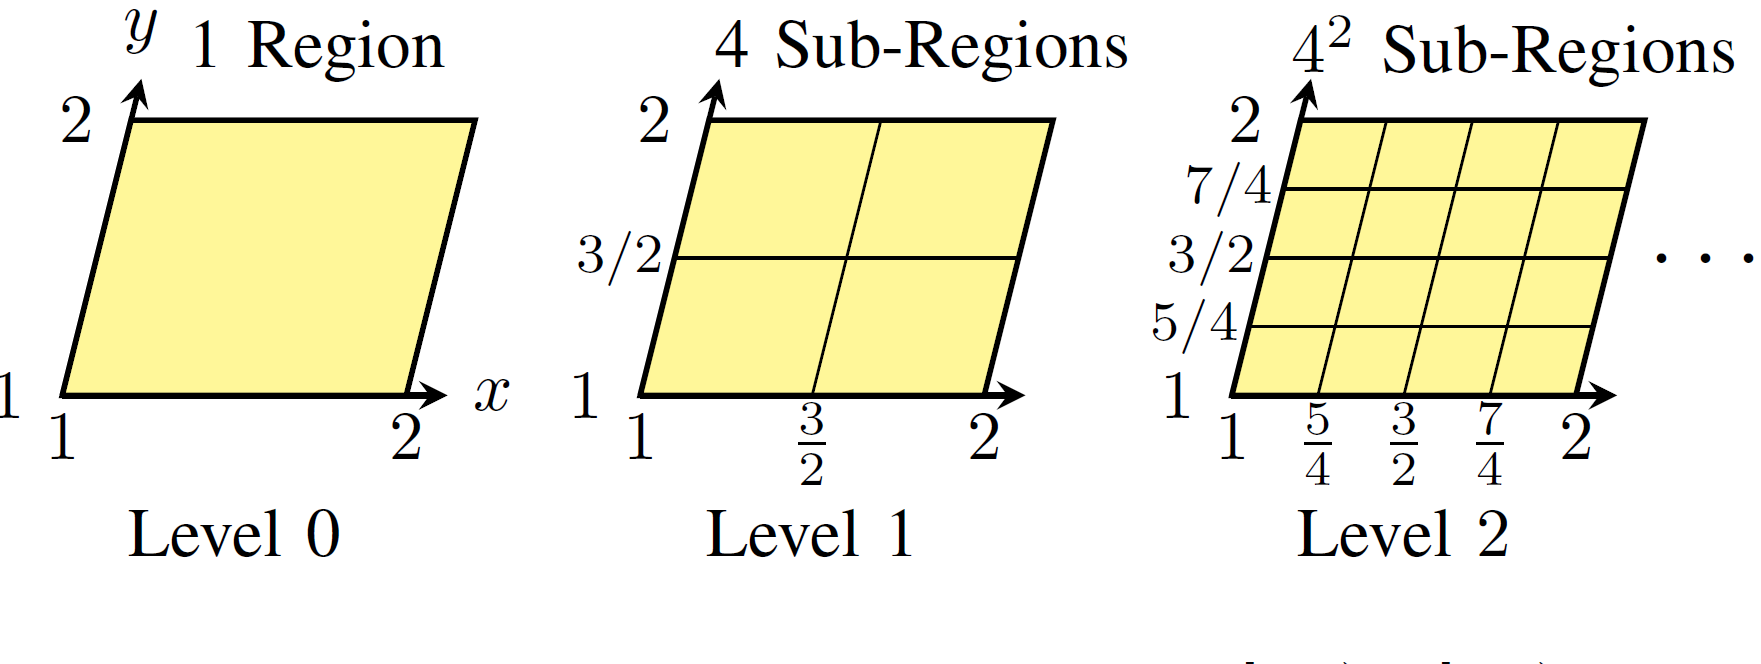
\includegraphics[width=\columnwidth,trim=0 19pt 0 0,clip]{pictures/Figure 2.png}
\caption{Mantissa partition at successive levels. The leading fraction bits
select a cell; its midpoint determines both local planes.}
\label{fig:partition}
\end{figure}

The same divider follows by combining a reciprocal tangent with the OAM
plane. The reciprocal tangent at $k_y$ is
$g(y)=2/k_y-y/k_y^2$. Substituting
$\widehat m=-k_xk_y+k_yx+k_xy$ into $xg(y)$ gives
\begin{equation}
\begin{aligned}
xg(y)&=\frac{2x}{k_y}-\frac{xy}{k_y^2}\\
&\approx\frac{2x}{k_y}-\frac{-k_xk_y+k_yx+k_xy}{k_y^2}\\
&=\frac{k_xk_y+k_yx-k_xy}{k_y^2}.
\end{aligned}
\label{eq:oamlink}
\end{equation}
Replacing $x,y$ by their centered forms recovers
Eq.~\eqref{eq:divplane}. Thus the connection is algebraic, rather than a
similarity between two separately fitted coefficient tables.

\subsection{Direct Evaluation at a Selected Level}
The partition in Fig.~\ref{fig:partition} can be evaluated recursively.
If $P_i$ is the plane at level $i$, define
$\Delta P_i=P_i-P_{i-1}$. Then
\begin{equation}
P_n=P_0+\sum_{i=1}^{n}\Delta P_i.
\label{eq:corrections}
\end{equation}
STDM instead decodes the final cell and evaluates $P_n$ once.
Before precision reduction, the two forms are algebraically equivalent.
Direct evaluation avoids intermediate correction generators and additions
when only one level is required.

The selected level controls the partition, residual width, and coefficient
precision. It is an implementation parameter, not an additional input to the
finished circuit. The operation bit remains live and selects the DIV or MUL
coefficients for that level. This distinction matters when interpreting area:
each reported unit contains one partition level and supports either operation.

Centering also exposes why reduced precision can save hardware.
The residual spans one cell width, rather than the full mantissa range.
After low bits are removed, its independent width decreases with finer
partitioning. The cost of its products can therefore fall even though more
coefficient entries are needed. The coefficient table and product widths must
be considered together; the number of cells alone does not determine area.

The retained field can be derived directly from the FP32 fraction.
Let $m_x=2^{23}x$ be the unsigned 24-bit mantissa integer and let
$j_x$ contain its lower $23-n$ bits. Within a selected cell,
\begin{equation}
\begin{aligned}
m_x&=2^{23}+i_x2^{23-n}+j_x,\\
R_x&=j_x-2^{22-n}.
\end{aligned}
\label{eq:localinteger}
\end{equation}
The midpoint offset is a power of two, so the centered integer requires only
$23-n$ independent signed bits. This representation gives the same midpoint
for every operand in the cell and avoids a general midpoint subtractor.
The corresponding expressions for $y$ are identical.

\section{Shared Circuit Implementation}
\subsection{Residual Precision and Coefficient Absorption}
Let $R_x=2^{23}r_x$ and $R_y=2^{23}r_y$ be signed Q23 integers.
Dropping $D_r$ low bits produces
\begin{equation}
\rho_x=\left\lfloor R_x/2^{D_r}\right\rfloor,\qquad
\rho_y=\left\lfloor R_y/2^{D_r}\right\rfloor.
\label{eq:rho}
\end{equation}
Each retained residual has $b=23-n-D_r$ signed bits. The arithmetic uses
these short integers, while the interface remains FP32.

A straightforward divider would form the three-term plane and multiply its
sum by a reciprocal coefficient. STDM distributes that coefficient over the
plane before generating RTL. Let $\bar c$ be a quantized reciprocal-square
coefficient. With $S$ fractional bits for each slope, define
\begin{equation}
\begin{aligned}
A_M&=\operatorname{round}(2^S k_y),&
B_M&=\operatorname{round}(2^S k_x),\\
A_D&=\operatorname{round}(2^S\bar c k_y),&
B_D&=\operatorname{round}(2^S\bar c k_x).
\end{aligned}
\label{eq:slopes}
\end{equation}
Here $M$ and $D$ identify the operation. Since the residual step is
$\Delta_r=2^{D_r-23}$, an integer product $A\rho$ represents
$A\rho\,2^{D_r-23-S}$. The constant must use the same scale,
so its fractional precision is
\begin{equation}
F=S+23-D_r.
\label{eq:scale}
\end{equation}
The two integer functions are
\begin{align}
Q_M&=T_M+A_M\rho_x+B_M\rho_y,\label{eq:signedmul}\\
Q_D&=T_D+A_D\rho_x-B_D\rho_y,\label{eq:signeddiv}\\
T_M&=\operatorname{round}\bigl(2^F(k_xk_y+b_M)\bigr),\nonumber\\
T_D&=\operatorname{round}(2^F\bar c k_xk_y).\nonumber
\end{align}
Their represented mantissas are $Q_M2^{-F}$ and $Q_D2^{-F}$.
The output integer is shifted by $23-F=D_r-S$ to restore Q23
alignment before normalization. This fixed shift requires wiring.

Residual truncation biases multiplication because both discarded terms have
the same sign. Write $\widetilde r_x=r_x-\epsilon_x$ and
$\widetilde r_y=r_y-\epsilon_y$, with
$0\leq\epsilon_x,\epsilon_y<\Delta_r$. The plane error is
$-k_y\epsilon_x-k_x\epsilon_y$.
For inputs approximately uniform within a cell,
$\mathrm{E}[\epsilon_x]\simeq\mathrm{E}[\epsilon_y]\simeq\Delta_r/2$.
We therefore include
\begin{equation}
b_M=(k_x+k_y)\Delta_r/2
\label{eq:bias}
\end{equation}
in $T_M$. It requires no separate correction adder.

Coefficient absorption removes the subsequent reciprocal multiplier, but
rounding the absorbed coefficients can change the approximation.
We treat that rounding separately from the exact recoding below.
The constant and slopes are generated offline for each cell and mode.
Synthesis implements their selection as combinational logic.

\subsection{Exact Unsigned Residual Recoding}
Signed products and DIV subtraction remain in
Eqs.~\eqref{eq:signedmul} and~\eqref{eq:signeddiv}.
Let $H=2^{b-1}$ and introduce
\begin{equation}
u=\rho_x+H,\qquad v=\rho_y+H.
\label{eq:uv}
\end{equation}
Both fields range from zero to $2^b-1$. Because each midpoint lies at
the center of a binary interval, $u$ and $v$ are already present in the
retained local fraction bits. For a fraction vector $f_x[22:0]$,
$u=f_x[22-n:D_r]$; $v$ is selected in the same way.
No arithmetic is needed to construct them.

In fact, Eq.~\eqref{eq:localinteger} gives
$\rho_x=\lfloor j_x/2^{D_r}\rfloor-H$.
Adding $H$ therefore recovers the retained local bits exactly.
This also covers negative residuals: removing low bits implements a floor,
not rounding toward zero. The distinction is essential to the constant
adjustments in Eqs.~\eqref{eq:unsignedmul} and~\eqref{eq:unsigneddiv}.
The DIV complement is applied only after selecting the retained field.
It consequently needs $b$ XOR gates rather than a complement over the
full FP32 mantissa.

For multiplication, substitution gives
\begin{equation}
\begin{aligned}
Q_M&=T'_M+A_Mu+B_Mv,\\
T'_M&=T_M-H(A_M+B_M).
\end{aligned}
\label{eq:unsignedmul}
\end{equation}
For division, use the $b$-bit complement
$\bar v=(2H-1)-v$. Since $\rho_y=H-1-\bar v$,
\begin{equation}
\begin{aligned}
Q_D&=T'_D+A_Du+B_D\bar v,\\
T'_D&=T_D-H(A_D+B_D)+B_D.
\end{aligned}
\label{eq:unsigneddiv}
\end{equation}
These are integer identities. The constant adjustments happen when the
tables are generated, so the circuit only selects the adjusted constant.
The selected L0--L3 coefficients yield nonnegative $T'$ values.
Both modes therefore use unsigned products and addition.

\begin{figure*}[t]
\centering
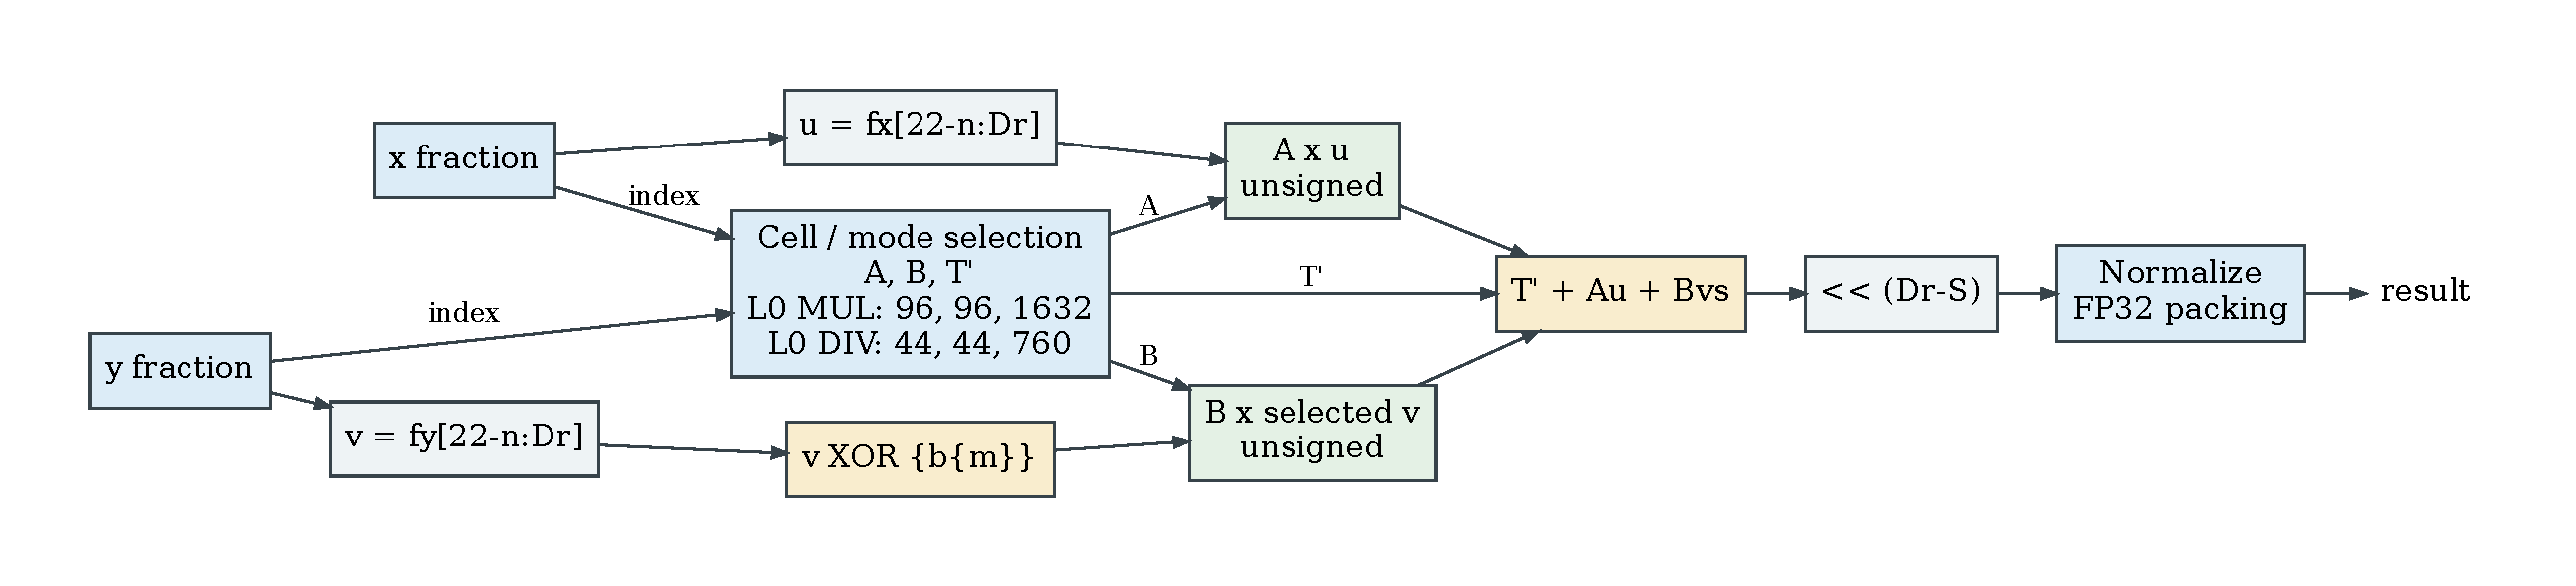
\includegraphics[width=\textwidth]{pictures/stdm_compact_circuit.pdf}
\caption{Shared mantissa circuit. Mode $m=1$ selects DIV and complements the
retained $y$ field; $m=0$ selects MUL. All coefficient values are integer codes.
The L0 example uses $D_r=18$, $S=6$, and $F=11$.}
\label{fig:circuit}
\end{figure*}

Figure~\ref{fig:circuit} shows the common datapath.
The cell indices and mode select $A,B,T'$.
One unsigned multiplier receives $u$; the other receives
$v\oplus\{b\{m\}\}$, where $m=1$ for DIV.
Their products and $T'$ feed the same adder. Alignment, normalization,
exponent correction, and FP32 packing follow.
The level-specific coefficient and residual widths are listed in
Table~\ref{tab:precision}. DIV and MUL use identical precision settings
within each shared unit.

\begin{table}[t]
\centering
\caption{Selected precision of the shared mantissa circuit}
\label{tab:precision}
\begin{tabular}{ccccc}
\toprule
Level & Residual drop $D_r$ & Width $b$ & $S$ & $F$\\
\midrule
L0 & 18 & 5 & 6 & 11\\
L1 & 16 & 6 & 4 & 11\\
L2 & 16 & 5 & 5 & 12\\
L3 & 16 & 4 & 4 & 11\\
\bottomrule
\end{tabular}
\end{table}

For example, L0 has $H=16$ and retains five bits per residual.
MUL selects $(A,B,T')=(96,96,1632)$, while DIV selects
$(44,44,760)$. Both sums are shifted left by 12 for Q23 alignment.
The shared circuit thus changes coefficient values and complements five bits
when the mode changes. It does not activate a separate divider core.

We checked the recoding against the signed integer forms over all retained
residual combinations and cell entries. RTL and gate-level regressions then
checked the packed outputs. The separate and shared implementations also
produce identical outputs for both modes at each selected level. These
checks establish equivalence of the implemented approximations; they do not
imply exact FP32 multiplication or division.

\begin{table*}[!t]
\centering\footnotesize
\renewcommand{\arraystretch}{1.15}
\caption{DIV-only accuracy and hardware results. STDM, PACE, PLSAD, and FPD2D
share the 200,000-pair accuracy set. ADP is normalized to exact DIV.}
\label{tab:div}
\setlength{\tabcolsep}{3pt}
\begin{tabular}{lrrrrrrrr}
\toprule
Design & MAE & MRED & RMSE & Area (\um) & Delay (ns) & Power (mW) & PDP (fJ) & Norm. ADP\\
\midrule
Exact DesignWare DIV & -- & -- & -- & 19604.52 & 9.750 & 1.89509 & 18477.43 & 1.0000\\
\midrule
STDM L0 & 0.042818 & 0.042856 & 0.056227 & 525.60 & 1.401 & 0.02103 & 29.47 & 0.0039\\
STDM L1 & 0.011796 & 0.011263 & 0.016233 & 809.64 & 1.685 & 0.03132 & 52.78 & 0.0071\\
STDM L2 & 0.003778 & 0.003568 & 0.005105 & 1030.32 & 1.940 & 0.03094 & 60.03 & 0.0105\\
STDM L3 & 0.002663 & 0.002577 & 0.003430 & 1149.12 & 2.006 & 0.03004 & 60.26 & 0.0121\\
\midrule
PACE L1 & 0.028163 & 0.025951 & 0.045176 & 990.00 & 2.214 & 0.04467 & 98.92 & 0.0115\\
PACE L2 & 0.015143 & 0.014859 & 0.022305 & 1551.60 & 2.362 & 0.07829 & 184.88 & 0.0192\\
PACE L3 & 0.005897 & 0.005608 & 0.009281 & 2271.96 & 2.821 & 0.13119 & 370.08 & 0.0335\\
PACE L4 & 0.003856 & 0.003816 & 0.006060 & 3150.72 & 2.987 & 0.18531 & 553.51 & 0.0492\\
\midrule
PLSAD ($m=8$) & 0.008975 & 0.008709 & 0.013227 & 659.88 & 1.738 & 0.02414 & 41.96 & 0.0060\\
FPD2D $8\times8,t=17$ & 0.005344 & 0.005282 & 0.006828 & 790.56 & 1.873 & 0.01981 & 37.09 & 0.0077\\
FPD2D $8\times8,t=16$ & 0.004054 & 0.004096 & 0.005134 & 869.76 & 1.962 & 0.02328 & 45.67 & 0.0089\\
FPD2D $8\times8,t=15$ & 0.003653 & 0.003735 & 0.004636 & 942.12 & 2.038 & 0.02660 & 54.22 & 0.0100\\
\midrule
FaNZeD & 0.031811 & 0.031130 & 0.046191 & 2775.96 & 4.968 & 0.08880 & 441.16 & 0.0721\\
TruncApp & 0.120105 & 0.119617 & 0.162391 & 4581.36 & 3.133 & 0.26136 & 818.77 & 0.0751\\
LEAD & 0.021750 & 0.020993 & 0.028841 & 6666.12 & 5.674 & 0.60630 & 3440.38 & 0.1979\\
QIAD & 0.005889 & 0.005880 & 0.006940 & 12097.80 & 8.074 & 0.95201 & 7686.66 & 0.5110\\
\bottomrule
\end{tabular}
\end{table*}

\subsection{Approximation Error and Coefficient Selection}
Partition error, residual truncation, and coefficient quantization have
different roles. For multiplication, the untruncated plane has the exact
remainder $xy-\widehat m=r_xr_y$, hence
$|xy-\widehat m|\leq2^{-2n-2}$. For division,
direct substitution gives
\begin{equation}
e=\frac{x}{y}-\widehat d
 =\frac{r_y(k_xr_y-k_yr_x)}{k_y^2y}.
\label{eq:exacterror}
\end{equation}
Since $1\leq k_x,k_y,y<2$, the residual bound implies
$|e|\leq4^{-n}$. Thus each partition refinement reduces this conservative
bound by a factor of four. It describes the tangent approximation before
precision reduction.

With exact $c=k_y^{-2}$, residual truncation changes the divider error by
\begin{equation}
e^{(r)}-e=c(k_y\epsilon_x-k_x\epsilon_y).
\label{eq:truncerror}
\end{equation}
The two contributions can cancel. A simple bound is
$|e^{(r)}-e|<c(k_x+k_y)\Delta_r$.
MUL instead adds both discarded contributions, which motivates
Eq.~\eqref{eq:bias}. The compensation corrects their estimated mean, not
each individual result.

To include coefficient error, define ideally scaled coefficients
$A_D^*=2^Sck_y$, $B_D^*=2^Sck_x$, and
$T_D^*=2^Fck_xk_y$. Let
$\delta_A=A_D-A_D^*$, $\delta_B=B_D-B_D^*$, and
$\delta_T=T_D-T_D^*$. For the implemented integer coefficients,
\begin{equation}
e^{(q)}-e^{(r)}
=-2^{-F}(\delta_T+\delta_A\rho_x-\delta_B\rho_y).
\label{eq:coefficienterror}
\end{equation}
The minus sign follows from defining error as exact minus approximate.
This expression includes reciprocal quantization and rounding after
absorption. The H recoding contributes no additional error.
Measured errors use the final FP32 outputs, including normalization and
packing.

The nearest reciprocal code need not minimize the final error.
For an intermediate plane $w$, let $e_0=x/y-C_0w$.
Replacing $C_0$ by $C_0+\delta$ gives
\begin{equation}
\mathrm{E}[e^2]=\mathrm{E}[e_0^2]
-2\delta\,\mathrm{E}[e_0w]+\delta^2\mathrm{E}[w^2].
\label{eq:calibration}
\end{equation}
The cross term couples reciprocal error to plane error.
Our earlier L0 calibration selects the Q0.7 code 59 rather than the nearest
code 57. The stored integer 59 represents $59/128$; it is subsequently
absorbed into $A_D,B_D,T_D$. This inherited choice is not a claim that 59
remains the unique optimum after every change in absorbed precision.
The measured results below correspond to the selected final coefficients.

\begin{figure}[t]
\centering
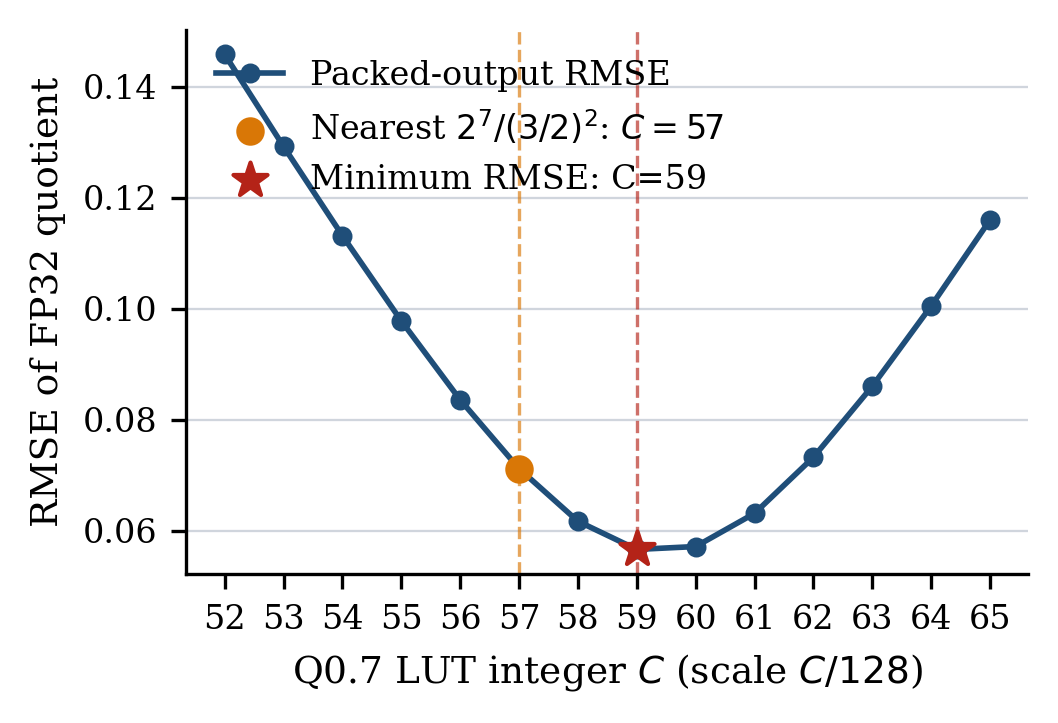
\includegraphics[width=\columnwidth]{pictures/l0_q07_coefficient_sweep.png}
\caption{L0 reciprocal calibration before coefficient absorption.
Code $C$ represents $C/128$. The minimum packed-output RMSE occurs at
$C=59$, rather than the nearest reciprocal code, $C=57$.
Final absorbed designs are evaluated separately in Table~\ref{tab:div}.}
\label{fig:calibration}
\end{figure}

Figure~\ref{fig:calibration} illustrates that calibration step. Once the
reciprocal is absorbed, $S$ controls a second quantization: it sets the grid
on which the two slopes are represented. The constant uses the scale in
Eq.~\eqref{eq:scale}, so changing $S$ can also change its rounding.
These changes need not move the errors in the same direction.
For example, the selected L0 $S=6$ point has slightly higher RMSE than
the earlier $S=7$ point, but lower MAE, MRED, and hardware cost.
We retain this tradeoff rather than treating fewer coefficient bits as an
automatic loss in every error metric.

Equation~\eqref{eq:coefficienterror} also gives a bound over the retained
integer domain:
\begin{equation}
|e^{(q)}-e^{(r)}|
\leq 2^{-F}\bigl(|\delta_T|+H(|\delta_A|+|\delta_B|)\bigr).
\label{eq:quantbound}
\end{equation}
The slope errors are weighted by the residual range.
This explains why coefficient precision and residual precision must be
selected together. A finer cell reduces that range, but may require more
selection logic. The final choice uses measured error and synthesized cost;
the bound identifies the error sources without predicting a unique
hardware optimum.



\section{Evaluation}
\subsection{Method and Comparison Scope}
We use Design Compiler U-2022.12-SP7 and PrimeTime U-2022.12-SP5 with the
TSMC 65-nm typical CCS library. All circuits are combinational, with a
10-ns virtual clock, 20-ps I/O delays, \texttt{INVD0} input driver, and
0.004 output load. Power uses input probability 0.5 and toggle rate 0.1
per period. PDP and ADP denote power--delay and area--delay products;
PDP is a vectorless estimate, not application energy.

PPA includes FP32 sign, exponent, normalization, and packing.
The evaluated domain contains normal finite operands without exponent
overflow or underflow; exceptional values and subnormals are excluded.
PACE retains the supplied mantissa RTL and normal-FP32 wrapper.
PLSAD and FPD2D are local reconstructions. PLSAD uses ten-bit inputs,
eight planes, and an eight-bit exact upper adder. FPD2D uses an $8\times8$
partition and reproduced coefficient optimization because its printed table
contains anomalous cells. FaNZeD, TruncApp, LEAD, and QIAD retain the
existing local adaptations; LEAD is a verified combinational unroll.

STDM, PACE, PLSAD, and FPD2D use the same 200,000 positive normalized
FP32 pairs. Errors are measured after FP32 packing. Other divider rows
retain their earlier 10,000-pair results for context; all PPA uses the
common flow.

The exact combined reference contains parallel \texttt{DW\_fp\_div} and
\texttt{DW\_fp\_mult} operators with an output selector. It provides the cost
of supporting both exact FP32 operations under the same interface, rather than
an accuracy-matched competitor. No prior approximate combined unit is placed
in the table: SIMDive has an integer SIMD FPGA interface, while the other fused
units reviewed in Section~II compute exact results with different timing
contracts.

\subsection{DIV-Only Accuracy and Cost}
Table~\ref{tab:div} shows the four STDM divider specializations.
Accuracy improves from L0 to L3 in all three reported metrics.
L0 has the smallest area and delay, but is less accurate than PACE L1.
STDM L1--L3 have lower MAE, MRED, and RMSE than PACE L2--L4,
respectively, with lower area, delay, and power in each pair.

The more specialized surface-fitting dividers present a closer comparison.
PLSAD lies between STDM L1 and L2 in error and occupies less area than L1.
FPD2D $t=16$ nearly matches L2 RMSE while using less area and power.
STDM L2 is slightly faster and has lower MRED, but its ADP remains higher.
At L3, STDM improves all three error measures over the evaluated FPD2D
points, at greater area and power than $t=15$.
These results do not establish a universal DIV-only advantage.
They show the cost of the divider approximation that underlies the shared unit.



\clearpage
\twocolumn[
\begin{minipage}{\textwidth}
\centering\footnotesize
\renewcommand{\arraystretch}{1.15}
\captionof{table}{Combined DIV+MUL comparison and sharing ablation.
Separate and Shared have identical outputs within each level.
Both include one common normalization and FP32 output path. Percentages in
Shared rows are changes relative to Separate at the same level.}
\label{tab:combined}
\setlength{\tabcolsep}{2.1pt}
\begin{tabular}{llrrrrrrr}
\toprule
Design & Structure & DIV MRED & MUL MRED & Area (\um) & Delay (ns) & Power (mW) & PDP (fJ) & ADP (\um\,ns)\\
\midrule
Exact DesignWare & DIV+MUL & -- & -- & 24025.68 & 9.856 & 2.08421 & 20541.66 & 236793.50\\
\midrule
STDM L0 & Separate & 0.042856 & 0.032453 & 911.88 & 1.649 & 0.03451 & 56.89 & 1503.44\\
 & Shared & 0.042856 & 0.032453 & \shortstack{891.36\\(-2.3\%)} & \shortstack{1.836\\(+11.3\%)} & \shortstack{0.03415\\(-1.0\%)} & \shortstack{62.71\\(+10.2\%)} & \shortstack{1636.94\\(+8.9\%)}\\
STDM L1 & Separate & 0.011263 & 0.007903 & 1429.20 & 2.005 & 0.05746 & 115.23 & 2866.09\\
 & Shared & 0.011263 & 0.007903 & \shortstack{1183.32\\(-17.2\%)} & \shortstack{2.136\\(+6.5\%)} & \shortstack{0.03932\\(-31.6\%)} & \shortstack{83.99\\(-27.1\%)} & \shortstack{2527.95\\(-11.8\%)}\\
STDM L2 & Separate & 0.003568 & 0.002687 & 1796.40 & 2.271 & 0.06416 & 145.71 & 4079.48\\
 & Shared & 0.003568 & 0.002687 & \shortstack{1454.40\\(-19.0\%)} & \shortstack{2.401\\(+5.7\%)} & \shortstack{0.03797\\(-40.8\%)} & \shortstack{91.17\\(-37.4\%)} & \shortstack{3492.15\\(-14.4\%)}\\
STDM L3 & Separate & 0.002577 & 0.001901 & 2196.72 & 2.374 & 0.06850 & 162.62 & 5215.28\\
 & Shared & 0.002577 & 0.001901 & \shortstack{1794.96\\(-18.3\%)} & \shortstack{2.509\\(+5.7\%)} & \shortstack{0.03944\\(-42.4\%)} & \shortstack{98.95\\(-39.2\%)} & \shortstack{4503.29\\(-13.7\%)}\\
\bottomrule
\end{tabular}
\end{minipage}
\vspace{12pt}
]
\balance
\subsection{Combined Unit and Sharing Benefit}
Table~\ref{tab:combined} combines the full-unit comparison with the sharing
ablation. In Separate, DIV and MUL have independent mantissa cores.
A selector chooses their result before common normalization and FP32 packing.
In Shared, cell decoding, both residual products, and accumulation are also
shared. Both structures use coefficient absorption and H recoding with
matching precision. This isolates the hardware effect of sharing without
changing either operation's outputs.

At L1--L3, sharing reduces area by 17.2--19.0\%, power by 31.6--42.4\%,
and ADP by 11.8--14.4\%. Delay increases by at most 6.5\%.
L0 behaves differently: area falls by 2.3\% and power by 1.0\%, but delay
increases by 11.4\%. Its ADP therefore rises by 8.9\%.
With only one cell, the separate L0 cores already use fixed coefficients.
Mode-dependent coefficient selection adds overhead to the shared path.
At higher levels, both structures need cell selection, and sharing saves a
larger portion of the arithmetic. Separate is preferable at L0 when minimum
ADP is the main objective.

At L3, STDM reduces area, delay, power, and ADP by 92.5\%, 74.5\%,
98.1\%, and 98.1\%, respectively, compared with exact DIV+MUL.

The measured benefit is strongest when one execution resource must support
both operations without simultaneous issue. A design requiring independent
DIV and MUL throughput would need separate resources or replicated units.
The current evidence covers combinational hardware cost and arithmetic error.
Application-level quality and activity-based energy remain to be evaluated.

\clearpage
\nobalance
\raggedbottom
\IEEEtriggeratref{9}
\begin{thebibliography}{21}
\bibitem{chen2010kmeans}
T.-W. Chen and S.-Y. Chien, ``Bandwidth adaptive hardware architecture of
K-means clustering for video analysis,'' \emph{IEEE Trans. Very Large Scale
Integr. (VLSI) Syst.}, vol. 18, no. 6, pp. 957--966, 2010,
doi: 10.1109/TVLSI.2009.2017543.
\bibitem{yao2024nlms}
C.-Y. Yao and Y.-Z. Huang, ``The design of the NLMS adaptive filters using the
fast-division approximation with CSD encoded divisors,'' \emph{IEEE Trans.
Circuits Syst. II, Exp. Briefs}, 2024, doi: 10.1109/TCSII.2023.3332692.
\bibitem{ebrahimi2020simdive}
Z. Ebrahimi, S. Ullah, and A. Kumar, ``SIMDive: Approximate SIMD soft
multiplier-divider for FPGAs with tunable accuracy,'' in \emph{Proc. GLSVLSI},
2020.
\bibitem{chen2004fused}
C. Chen, H.-L. Yen, and M.-H. Sheu, ``Design of a cost-effective
multiplier/divider fused unit for floating-point arithmetic,''
\emph{Int. J. Electr. Eng.}, vol. 11, no. 3, pp. 239--246, 2004.
\bibitem{kwon2004diva}
T.-J. Kwon, J.-S. Moon, J. Sondeen, and J. Draper, ``A 0.18-$\mu$m
implementation of a floating-point unit for a processing-in-memory system,''
in \emph{Proc. IEEE ISCAS}, 2004, vol. 2, pp. II-453--II-456,
doi: 10.1109/ISCAS.2004.1329306.
\bibitem{gaislergrfpu}
Frontgrade Gaisler, ``GRFPU: High-performance IEEE-754 floating-point unit,''
[Online]. Available: https://www.gaisler.com/products/ieee-754-floating-point-unit.
\bibitem{chen2020oam}
C. Chen, S. Yang, W. Qian, M. Imani, X. Yin, and C. Zhuo,
``Optimally approximated and unbiased floating-point multiplier with runtime
configurability,'' in \emph{Proc. IEEE/ACM ICCAD}, 2020, pp. 1--9.
\bibitem{chen2015nonrestoring}
L. Chen, J. Han, W. Liu, and F. Lombardi, ``Design of approximate unsigned
integer non-restoring divider for inexact computing,'' in \emph{Proc. GLSVLSI},
2015, pp. 51--56, doi: 10.1145/2742060.2742063.
\bibitem{hashemi2016dynamic}
S. Hashemi, R. I. Bahar, and S. Reda, ``A low-power dynamic divider for
approximate applications,'' in \emph{Proc. DAC}, 2016, pp. 1--6,
doi: 10.1145/2897937.2897965.
\bibitem{vahdat2017truncapp}
S. Vahdat, M. Kamal, A. Afzali-Kusha, M. Pedram, and Z. Navabi,
``TruncApp: A truncation-based approximate divider for energy efficient DSP
applications,'' in \emph{Proc. DATE}, 2017,
doi: 10.23919/DATE.2017.7927254.
\bibitem{saadat2019fanzed}
H. Saadat, H. Javaid, and S. Parameswaran, ``Approximate integer and
floating-point dividers with near-zero error bias,'' in \emph{Proc. DAC},
2019, doi: 10.1145/3316781.3317773.
\bibitem{ratnaparkhi2022lead}
O. G. Ratnaparkhi and M. Rao, ``LEAD: Logarithmic exponent approximate divider
for image quantization application,'' in \emph{Proc. GLSVLSI}, 2022,
doi: 10.1145/3526241.3530323.
\bibitem{imani2019cade}
M. Imani, R. Garcia, A. Huang, and T. Rosing, ``CADE: Configurable approximate
divider for energy efficiency,'' in \emph{Proc. DATE}, 2019, pp. 586--589,
doi: 10.23919/DATE.2019.8715112.
\bibitem{melchert2019saadi}
J. Melchert, S. Behroozi, J. Li, and Y. Kim, ``SAADI-EC: A quality-configurable
approximate divider for energy efficiency,'' \emph{IEEE Trans. VLSI Syst.},
vol. 27, no. 11, pp. 2680--2692, 2019,
doi: 10.1109/TVLSI.2019.2926083.
\bibitem{oelund2023ilafd}
J. Oelund and S. Kim, ``ILAFD: Accuracy-configurable floating-point divider
using an approximate reciprocal and an iterative logarithmic multiplier,'' in
\emph{Proc. GLSVLSI}, 2023, pp. 639--644,
doi: 10.1145/3583781.3590262.
\bibitem{liu2023qiad}
H. Liu, M.-J. Wang, and M. Liu, ``QIAD: A quadratic interpolation approximate
divider,'' \emph{IEICE Electronics Express}, vol. 20, no. 11, 2023,
doi: 10.1587/elex.20.20230167.
\bibitem{wen2025pace}
C. Wen, H. Du, J. Wang, Z. Chen, L. Zhang, Q. Sun, and C. Zhuo,
``PACE: A piece-wise approximate floating-point divider with runtime
configurability and high energy efficiency,'' \emph{ACM Trans. Des. Autom.
Electron. Syst.}, vol. 30, no. 2, Art. 21, 2025,
doi: 10.1145/3706634.
\bibitem{wu2015curve}
L. Wu, ``A curve fitting approach for non-iterative divider design with
accuracy and performance trade-off,'' in \emph{Proc. NEWCAS}, 2015,
doi: 10.1109/NEWCAS.2015.7182097.
\bibitem{wu2024plsad}
C. Wu, W. Shi, Y. Yuan, Z. Zou, Z. Mo, and J. He,
``Area-delay-energy-efficient approximate dividers based on piecewise linear
fitting of surface,'' \emph{IEEE Trans. Circuits Syst. I, Reg. Papers},
vol. 71, no. 11, pp. 5017--5029, 2024,
doi: 10.1109/TCSI.2024.3425538.
\bibitem{dimeo2025fpd2d}
G. Di Meo, A. G. M. Strollo, D. De Caro, L. Tegazzini, and E. Napoli,
``Low-power high precision floating-point divider with bidimensional linear
approximation,'' \emph{IEEE Trans. Circuits Syst. I, Reg. Papers}, vol. 72,
no. 2, pp. 882--895, 2025, doi: 10.1109/TCSI.2024.3447830.
\bibitem{Ieee}
\emph{IEEE Standard for Floating-Point Arithmetic}, IEEE Standard 754-2008,
pp. 1--70, 2008.
\end{thebibliography}
\end{document}
